\section{Default filter set-up}
\label{sec:filt}

In this section we construct the effective filter response $R(\lambda)$ of the PAU bands and compute their 5-$\sigma$ limiting magnitudes, $m_{AB}(5\sigma)$.

\subsection{Nominal response}
PAUCam will mount two sets of filters: the Broad-Band~(BB) filters, composed of 6 bands \textit{ugrizY}\footnote{The $u$ band is assumed to be the same as the used in the USNO 40-in telescope at Flagstaff Station (Arizona) and its transmission can be obtained from \url{http://www.sdss.org/dr7/algorithms/standardstars/Filters/response.html}, while the rest are assumed to be the same as in the DECam mounted in the Blanco Telescope (CTIO, Chile).}%and their transmissions can be obtained from \url{http://des-docdb.fnal.gov:8080/cgi-bin/ShowDocument?docid=4295} (private link).}
, whose nominal (or theoretical) response $R^{theo}(\lambda)$ is shown on the top of Fig.~\ref{pau_theo_bands}, and the Narrow-Band~(NB) filters, shown on the bottom, which are composed of 40 top-hat adjacent bands with a rectangular width of 100\AA \ ranging from 4500\AA \ to 8500\AA. Since there is a technical limitation to construct such narrow top-hat bands, we relax the transition from 0 to the maximum response by adding two lateral wings of 25\AA \ width, resulting in a \textit{FWHM} of 125\AA. This induces an overlap of $\sim$25\% between contiguous bands. Additionally, we set the overall NB responses to match those from the ALHAMBRA survey instrument \citep{Moles2008}, which are comparable in technical specifications (although with a wider wavelength range, $\sim 310$\AA, transmission) and have similar coatings.
\begin{figure}
\centering
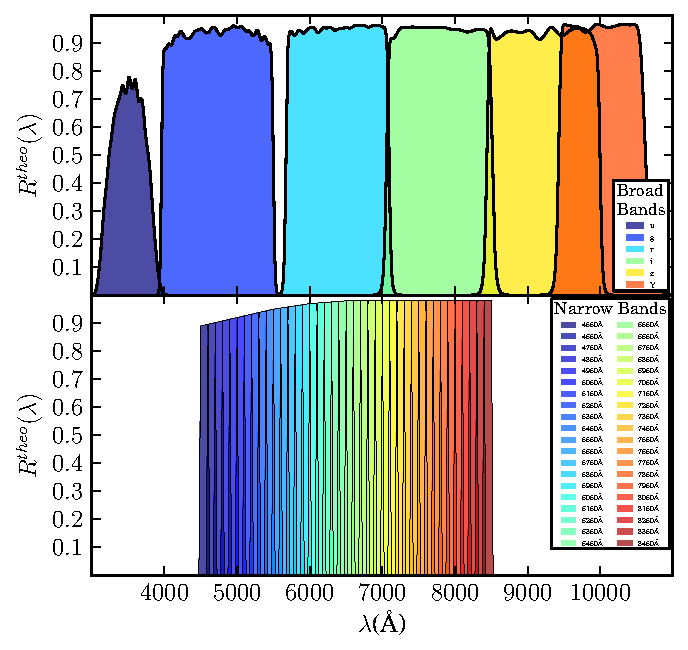
\includegraphics[width=84mm]{./plots/pau_theo_bands.pdf}
\caption{The nominal (or theoretical) response $R^{theo}(\lambda)$ of the \textit{ugrizY} PAU Broad Bands (top) and the 40 Narrow Bands (bottom). The \textit{u} band is the same as in the USNO 40-in telescope at Flagstaff Station (Arizona), while the \textit{grizY} are the same as in the DECam mounted in the Blanco Telescope (CTIO, Chile). The narrow-band filters have a 125\AA\ {\em FWHM} and overlap by 25\% with the adjacent bands. They are labeled on the plot through their central wavelength. Their overall response is set to match that of the ALHAMBRA survey bands.}
\label{pau_theo_bands}
\end{figure}

\subsection{Effective response}
The filter responses $R^{theo}(\lambda)$ in Fig. \ref{pau_theo_bands} are the nominal: this is the response that we would measure if light went only through the filter. Light also goes through the Earth's atmosphere, which absorbs part of the light, and then, also goes through the optics (mirror and corrector) of the telescope before getting into the filter. Moreover, the CCD detectors behind filters also are affected by a Quantum Efficiency (QE) response curve. Therefore, if we want to know the effective response of the filters, we will have to take into account all the transmission curves $T_i(\lambda)$ of these effects $i$. In our case, these curves are shown in the top plot of Fig. \ref{pau_effective_bands}. The QE curve (blue) corresponds to the measured QE of CCDs provided by Hammamatsu, the measured transmission curve of the telescope's optics (mirror + corrector) (green) corresponds to that from the William Herschel Telescope (WHT) optics, and the atmospheric transmission curve (red) is taken from the Apache Point Observatory (APO) at New Mexico. We assume that the APO atmosphere transmission is close enough to that at the Observatorio del Roque de los Muchachos (ORM) for the purpose of this study. The resulting effective response $R(\lambda)$ is derived with the expression:
\begin{eqnarray}
R(\lambda) &=& R^{theo}(\lambda) \prod_{i} T_i(\lambda) \nonumber \\
&=& R^{theo}(\lambda) \cdot T_{CCD}(\lambda) \cdot T_{opt}(\lambda) \cdot T_{atm}(\lambda).
%R(\lambda) = R^{theo}(\lambda) \prod_{i} T_i(\lambda).
\label{eff_filt}
\end{eqnarray}
The transmission of the WHT optics is less than 50\% in the whole wavelength range, so that the resulting effective responses are significantly reduced. On the other hand, the three transmission curves $T_i(\lambda)$ begin to fall when they enter the ultraviolet region ($\sim$3800\AA). Similarly, the CCDs QE drops as we approach the infrared region above $\sim$9000\AA. Overall, the $u$ and $Y$ broad bands are less efficient than the rest. This does not affect the NB, since their wavelength range are within these limits. Atmospheric telluric absorption bands, located between $\sim$700nm and $\sim$1$\mu$m, are also imprinted in the final response of the filters. This is particularly relevant for the NB since their typical width is similar to the width of these valleys. In particular, the profile of the narrow band with central wavelength at $\sim$7550\AA \ (orange) is drastically changed by the telluric absorption $A$-band. 
\begin{figure}
\centering
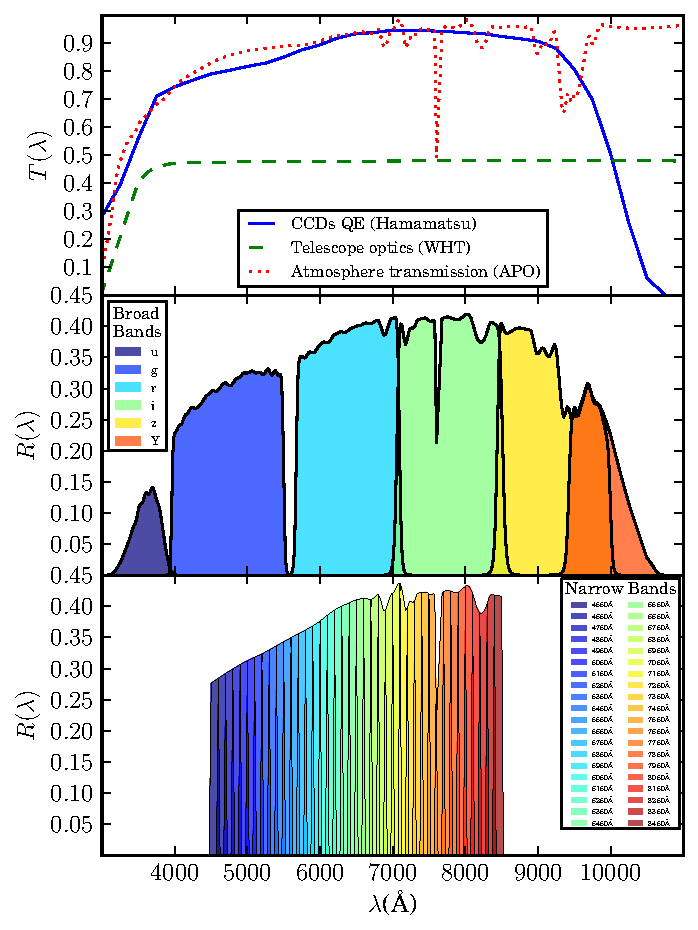
\includegraphics[width=84mm]{./plots/pau_effective_bands.pdf}
\caption{Top: the QE curve (blue) of the PAUCam CCDs, the transmission curve of the WHT optics (green), and the atmospheric transmission (red) at the APO (Apache Point Observatory), that affect the final response of the PAU bands. The two lower plots are the same as in Fig.~\ref{pau_theo_bands}, but after taking into account these additional transmission curves $T_i(\lambda)$ through Eq.~(\ref{eff_filt}). For the sake of clarity, we have rescaled the $y$-axes due to the low efficiency of the mirror's reflexion.}
\label{pau_effective_bands}
\end{figure}

\subsection{5-$\sigma$ limiting magnitudes}
Next, we compute the 5-$\sigma$ limiting magnitudes, $m_{AB}(5\sigma)$, for all the PAU bands in the AB photometric system\footnote{According to \citet{Hogg1996}, the apparent magnitude $m_{AB}$ in the AB system in a band with response $R(\lambda)$ for a source with spectral density flux $f(\nu)$ (energy per unit time per unit area per unit frequency) is defined as $m_{AB} \equiv-2.5\log_{10}\left[\int f(\nu) R(\nu){d\nu \over\nu} / \int \text{(3631Jy)} R(\nu){d\nu \over\nu}\right]$, where $1Jy = 10^{-23} erg\cdot s^{-1} \cdot cm^{-2} \cdot Hz^{-1}$ or $1.51 \cdot 10^7 photons\cdot m^{-2} \cdot s^{-1} \cdot {\lambda \over d\lambda}$ in wavelength space.} \citep{Oke1970}. This is the apparent magnitude whose Signal-to-Noise ratio, given by
\begin{equation}
{S \over N} = \sqrt{A \over \alpha^2}{N_{gal} \over \sqrt{N_{gal} + N_{sky} + n RN^2} },
\label{SN}
\end{equation}
is equal to 5, where 
\begin{eqnarray}
N_{gal} &=& 3631 \cdot 1.51\cdot10^7  \cdot 10^{-0.4m_{AB}} \cdot \left({\alpha^2\over A}\right) \cdot \nonumber \\
&\cdot& \pi\left({\phi \over 2}\right)^2 \cdot nt_R \cdot \int^{\infty}_0 R(\lambda) {d\lambda \over \lambda} \label{Ngal}, \label{Ngal} \\
N_{sky} &=& \alpha^2 \cdot \pi\left({\phi \over 2}\right)^2 \cdot nt_R \cdot \int^{\infty}_0 f_{sky}(\lambda) R(\lambda) d\lambda, \label{Nsky}
\end{eqnarray}
are the photons per pixel coming from the galaxy and the sky brightness  respectively, $\lbrace \phi, \alpha, RN, A, n \rbrace$ are the parameters of both the WHT and PAUCam instrument, whose values and description are given in Table \ref{PAU_parameters}, $f_{sky}(\lambda)$ is the spectral density flux per unit of aperture of the sky brightness, whose curve is on top of Fig.~\ref{pau_lim_mag}, and $t_R$ is the exposure time for the filter $R(\lambda)$. 
\begin{table}
\caption{Description and values of the WHT and PAUCam parameters used in (\ref{SN}), (\ref{Ngal}) and (\ref{Nsky}), to compute the Signal-to-Noise ratio ($S/N$).}
\vspace*{12pt}
\centering
\begin{tabular}{ccc}
\hline
 $\phi$ & Telescope mirror diameter & 4.2 m \\
$\alpha$ & Focal Plane Scale & 0.265 arcsec/pix \\
$RN$ & Read-out Noise & 5 electrons/pix \\
$A$ & Galaxy Aperture & 2 arcsec$^2$ \\
$n$ & \# of Exposures & 2 \\
\hline
\end{tabular}
\label{PAU_parameters}
\end{table}
All the filters intended for the photometry are arranged over the central part of the Focal Plane (FP) where vignetting is practically negligible. NB are distributed through 5 interchangeable trays. From the bluest to the reddest, each tray carries a group of 8 consecutive NB. This gives 5 trays $\times$ 8 NB $=$ 40 NB. 
Values for the exposure times $T_i$ of each tray are shown on the left column of Table \ref{PAU_Texp}. On the other hand, each BB filter is mounted into a dedicated tray with its particular exposure time, in such a way that NB and BB exposure times are completely decoupled. Values for the exposure times $t_R$ of each BB filter are shown on the right column of Table \ref{PAU_Texp}.
\begin{table}
\caption{Left: Exposure times $T_i$ for each PAUCam NB filter tray. The individual NB exposure times are equal to those of the tray where they are. Right: The BB exposure times. Exposure times $t_R$ per filter are also shown in the middle plot of Fig.~\ref{pau_lim_mag}.}
\vspace*{12pt}
\centering
\begin{tabular}{ccccc}
\multicolumn{2}{c}{NB tray $T_i$} & & \multicolumn{2}{c}{BB $t_R$} \\
\cline{1-2} \cline{4-5} 
$T_1$  & 45 sec & & u & 45 sec \\
$T_2$  & 45 sec & & g & 45 sec \\
$T_3$  & 50 sec & & r & 50 sec \\
$T_4$  & 60 sec & & i & 75 sec \\
$T_5$  & 75 sec & & z & 75 sec \\
       &        & & Y & 75 sec \\
\cline{1-2} \cline{4-5} 
\end{tabular}
\label{PAU_Texp}
\end{table}
The exposure times $t_R$ and the derived limiting magnitudes $m_{AB}(5\sigma)$ for each filter are also shown on the middle and bottom plots of Fig.~\ref{pau_lim_mag} respectively, in a color degradation for NB and in black for BB. 
\begin{figure}
\centering
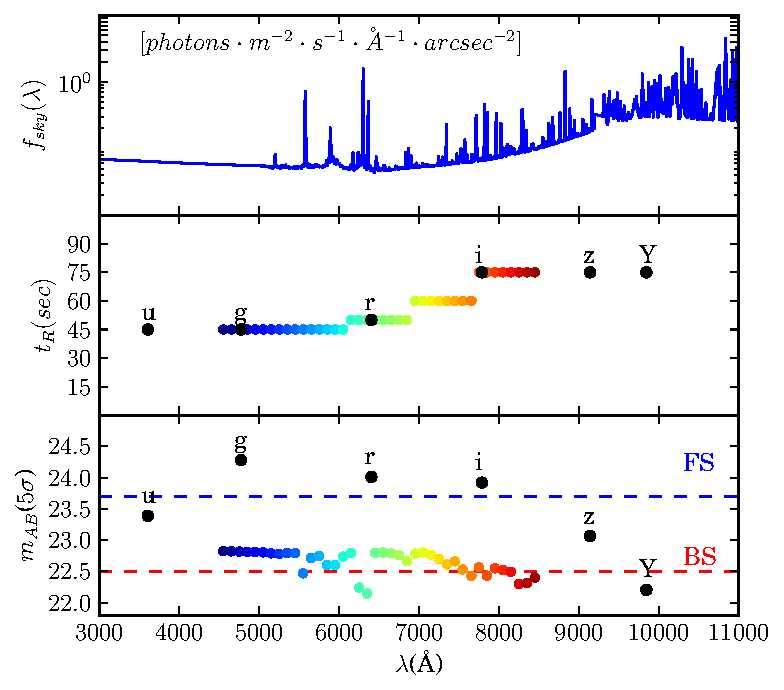
\includegraphics[width=84mm]{./plots/pau_lim_mag.pdf}
\caption{Top: a model of the spectral density flux of the sky brightness $f_{sky}(\lambda)$ at La Palma (day 7 on the lunar cycle) assuming an airmass of 1.0, used in (\ref{Nsky}). Middle: the exposure times $t_R$ for each PAU band used in (\ref{Ngal}) and (\ref{Nsky}). Bottom: the resulting limiting magnitudes $m_{AB}(5\sigma)$ for each band computed through (\ref{SN}), (\ref{Ngal}) and (\ref{Nsky}). Colored points correspond to Narrow Bands and black to Broad Bands.}
\label{pau_lim_mag}
\end{figure}
Since $f_{sky}(\lambda)$ increases with wavelength, exposure times $t_R$ for redder filters are also set to increase in order to compensate the noise introduced by the sky (note that the exposure times for the NB increase in steps, due to their arrangement in groups per tray). However, this increment is not enough to compensate the sky brightness as we can see with the descending $m_{AB}(5\sigma)$ with wavelength. Note that the $u$ band has a lower limiting magnitude compared with $g$ even being at shorter wavelengths. This is because the $u$ response is strongly affected by the transmission curves $T_i$. Furthermore, there are large drops in $m_{AB}(5\sigma)$ for the NB with central wavelength 5550\AA, 6250\AA \ and 6350\AA. This is  due to emission lines in the sky spectrum $f_{sky}(\lambda)$ at these wavelengths.
